\section{Results}\label{sec:results}
After applying the event pre-selection on the dataset, $280$ events are observed in the same-sign \mumu\ channel, $525$ in the same-sign \emu\ channel, and $149$ events in the trilepton channel (\threel).
The events are then sorted into ten categories depending on the output of the two BDT classifiers according to an optimized binning strategy, resulting in a one-dimensional histogram with ten bins.
The expected signal and background shapes for this distribution are then fit to the observed data in a maximum likelihood fit, simultaneously for all three channels and separately for the signal shapes for each of the 33 $\Ct/\CV$ coupling configuration points.

In each point, the \tH\ and \ttH\ production cross sections and the Higgs decay branching ratios are modified with the Higgs-top (\Ct) and Higgs-vector boson (\CV) coupling strength.
The Higgs-tau coupling strength modifier ($\kappa_\tau$) is assumed to be equal to \Ct.
% This includes modified branching ratios of $\PH\to\gamma\gamma$, $\PH\to\Z\gamma$, and $\PH\to\Pg\Pg$ with varying \Ct, and an accordingly adjusted overall Higgs decay width. % FIXME?
All other parameters are assumed to be at the values predicted by the standard model.
This implies that the combined signal shape is uniquely defined by the ratio of $\Ct/\CV$.
In the fit, the \tH\ and \ttH\ signal are then floated with a common signal strength modifier (defined as the ratio to the expected cross section) to produce a 95\% confidence level (C.L.) upper limit on the observed $\tH+\ttH$ cross section times the combined branching ratio of $\PH\to\W\W^*+\tautau+\Z\Z^*$.

The pre-fit BDT output distributions are shown in Fig.~\ref{fig:postfitshapes}, whereas Fig.~\ref{fig:finalbins} shows the post-fit categorized BDT output distributions obtained in the maximum likelihood fit to extract the limits.

\begin{figure}[!htb]
  \begin{center}
    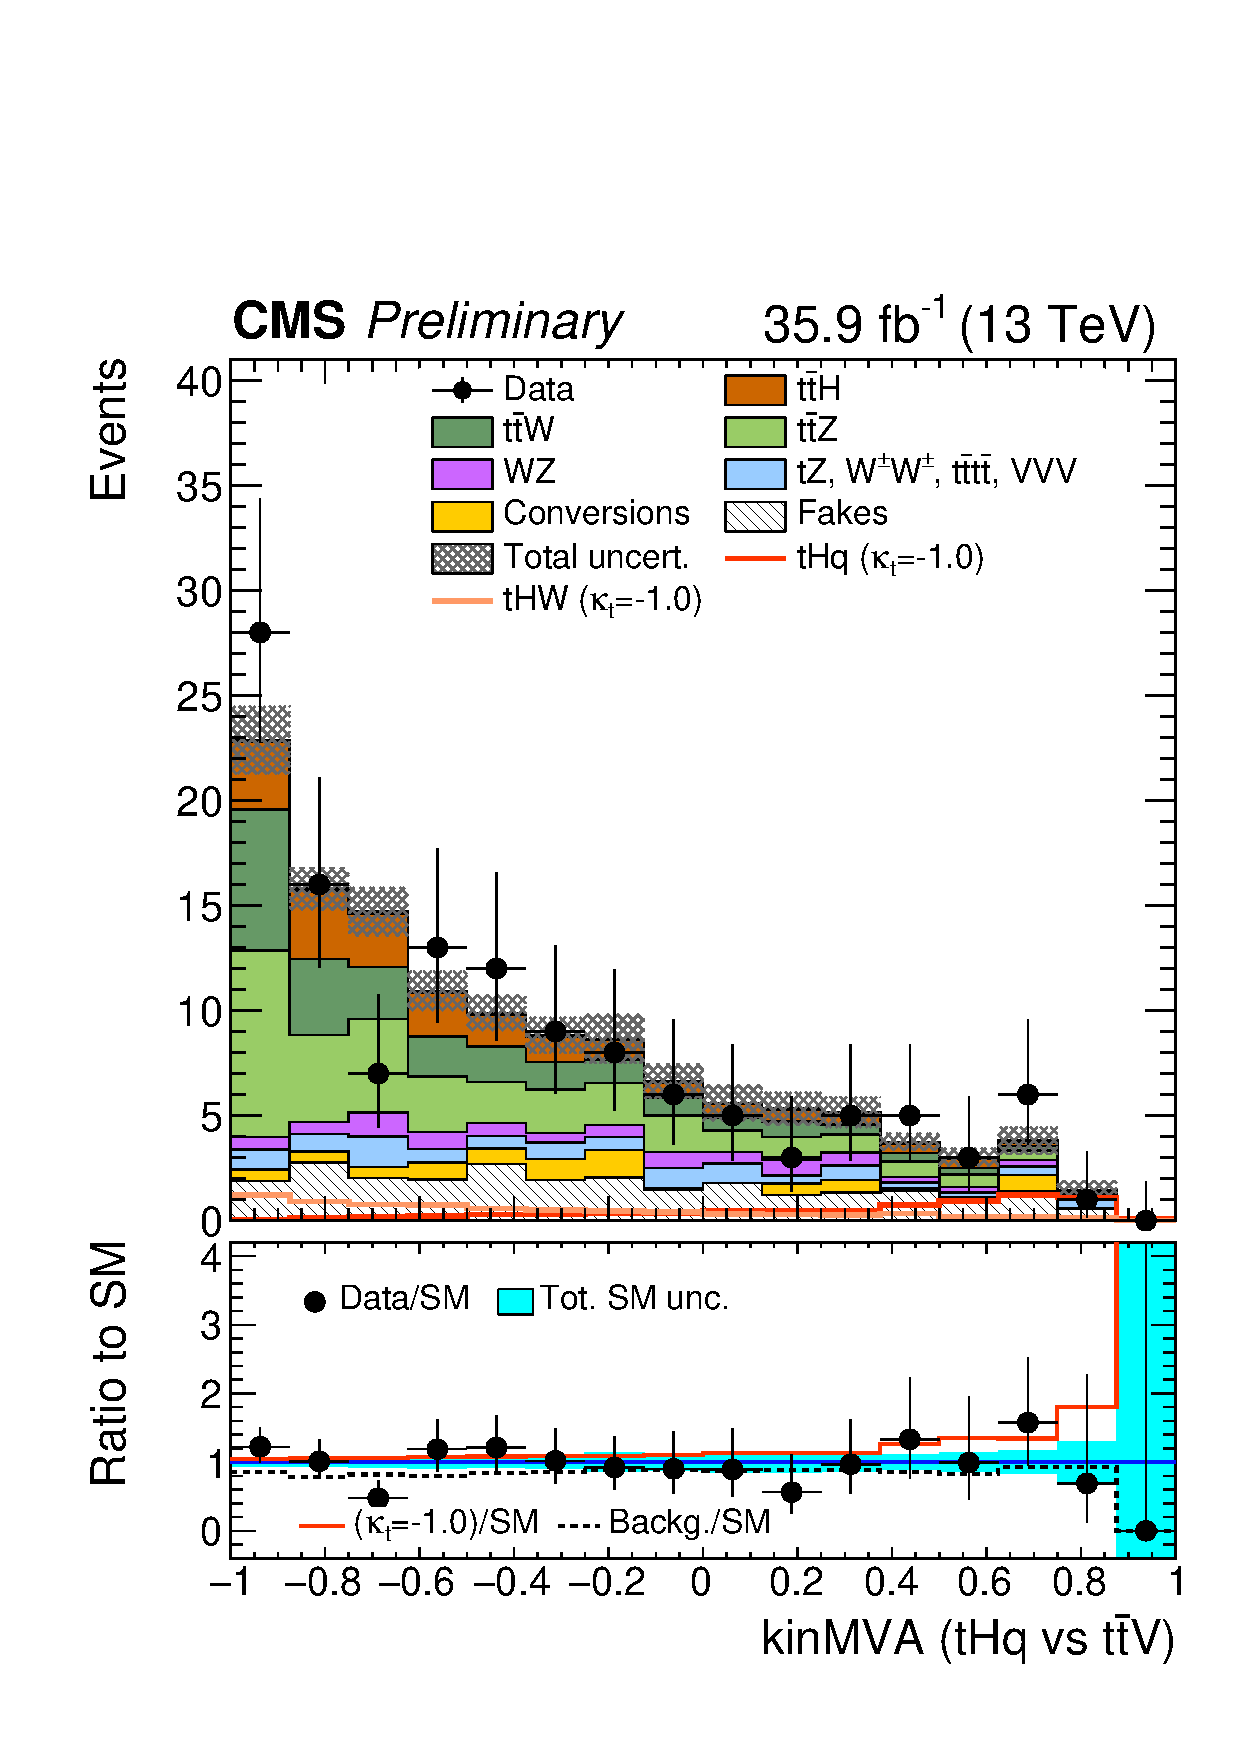
\includegraphics[width=0.32\textwidth]{Figures/polished/thqMVA_ttv_3l_40_3l.pdf} 
    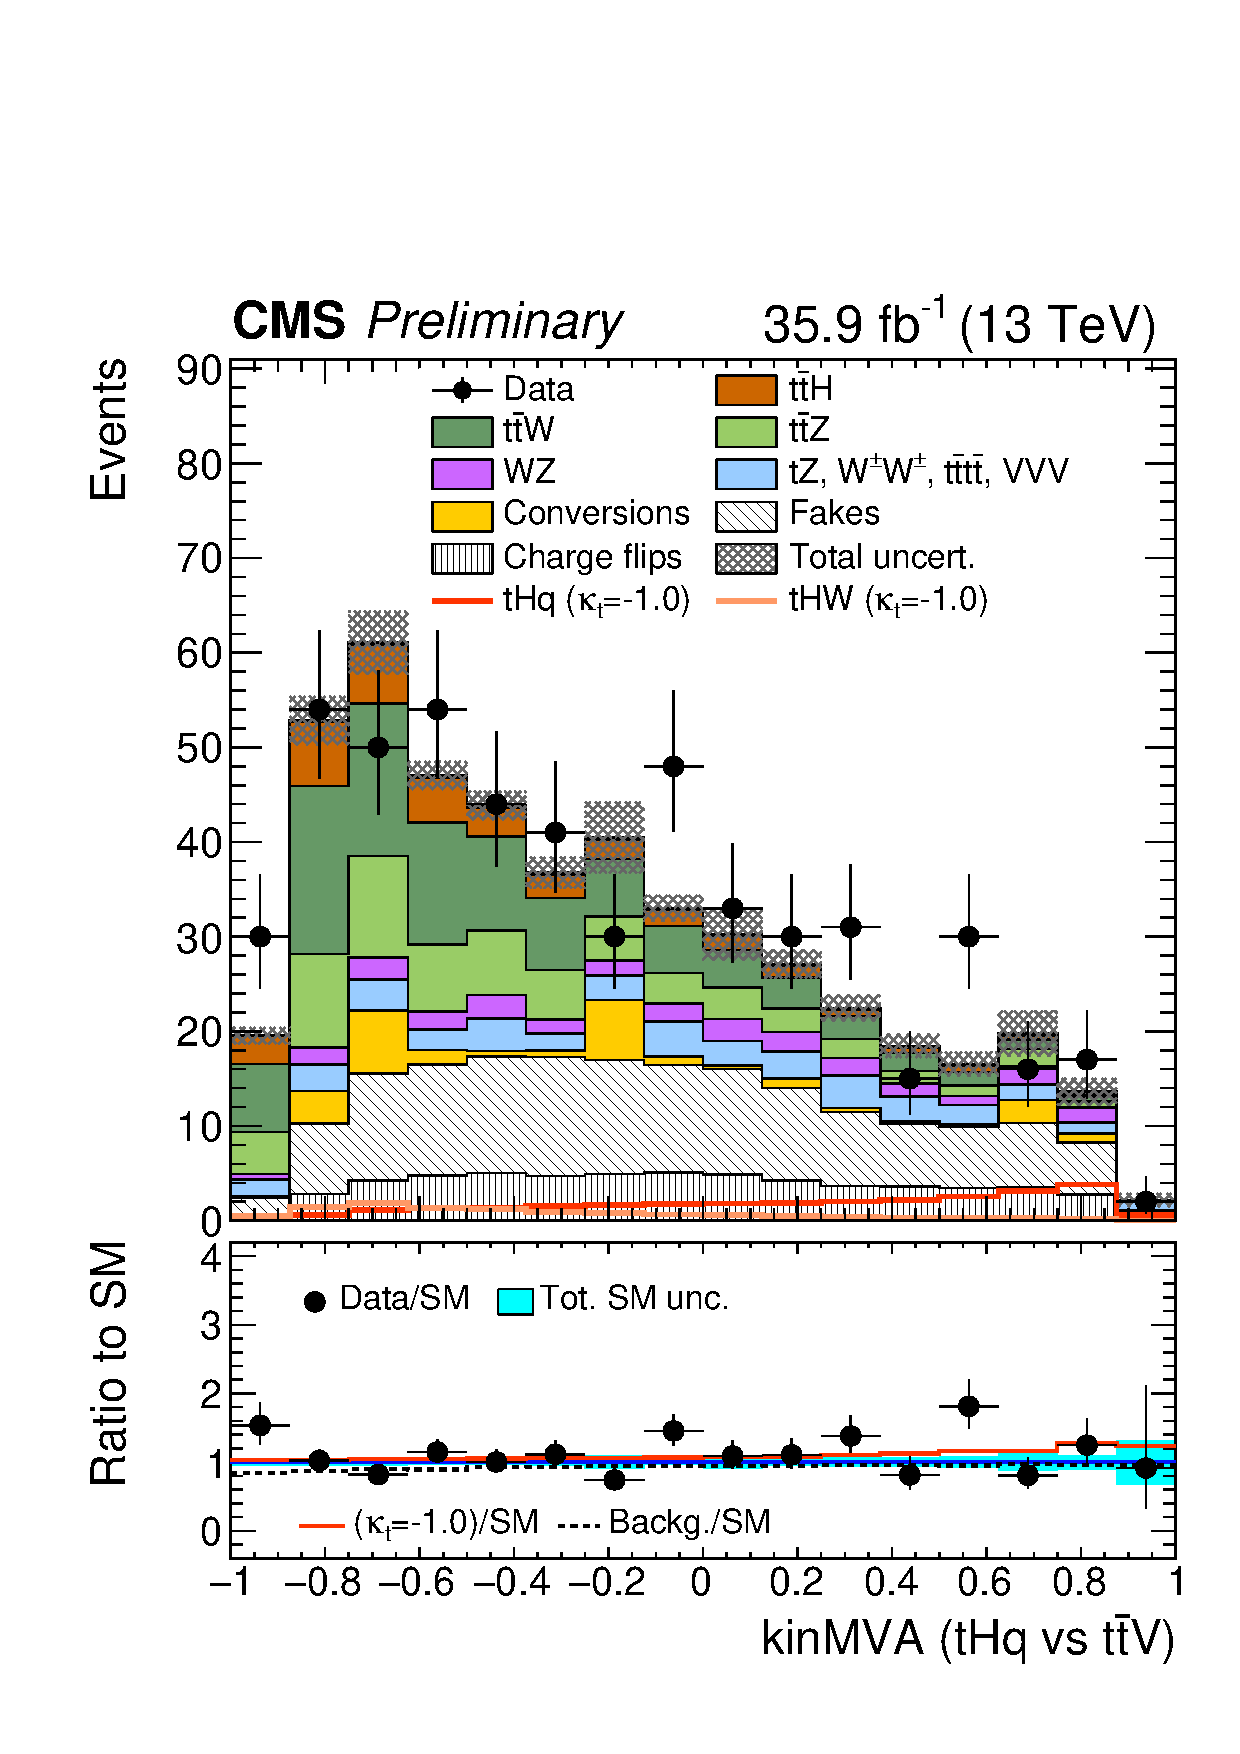
\includegraphics[width=0.32\textwidth]{Figures/polished/thqMVA_ttv_2lss_40_em.pdf}
    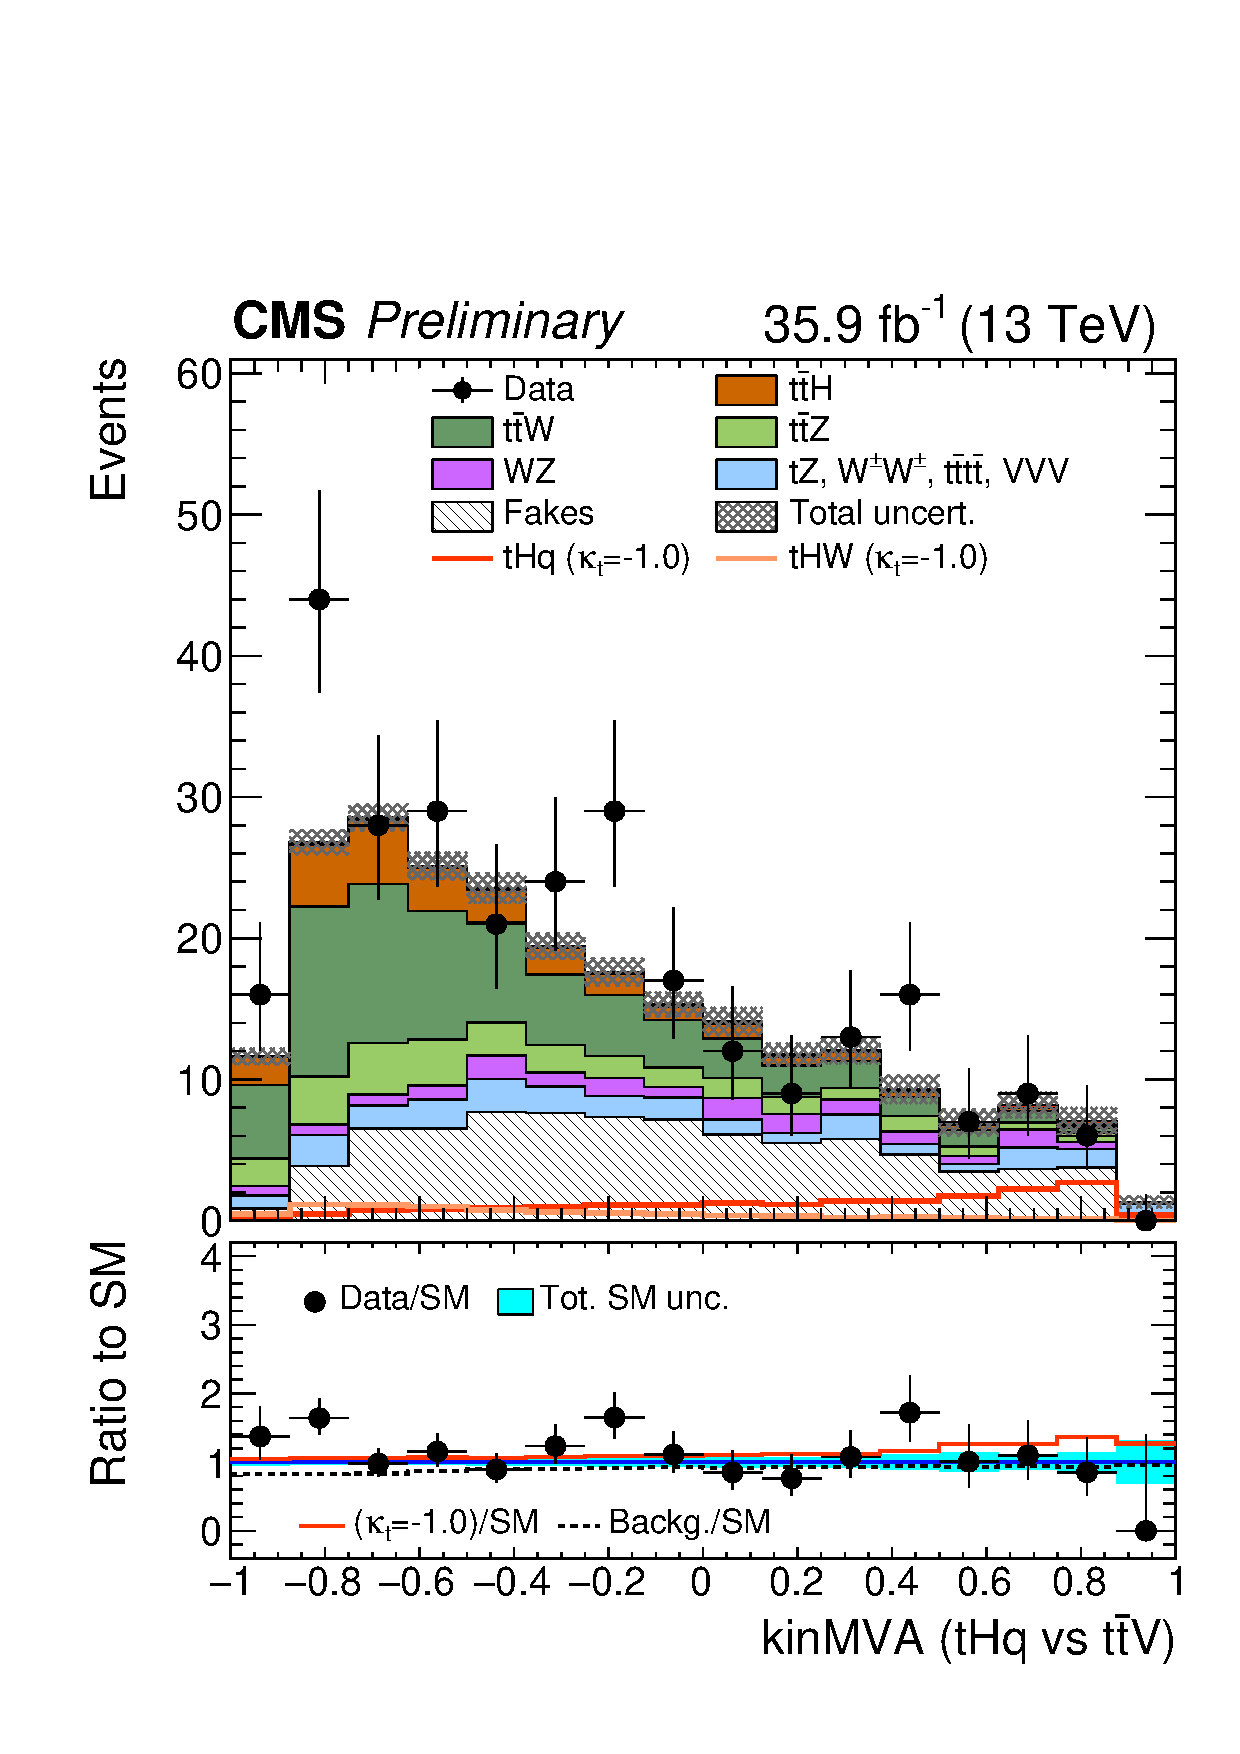
\includegraphics[width=0.32\textwidth]{Figures/polished/thqMVA_ttv_2lss_40_mm.pdf} \\
    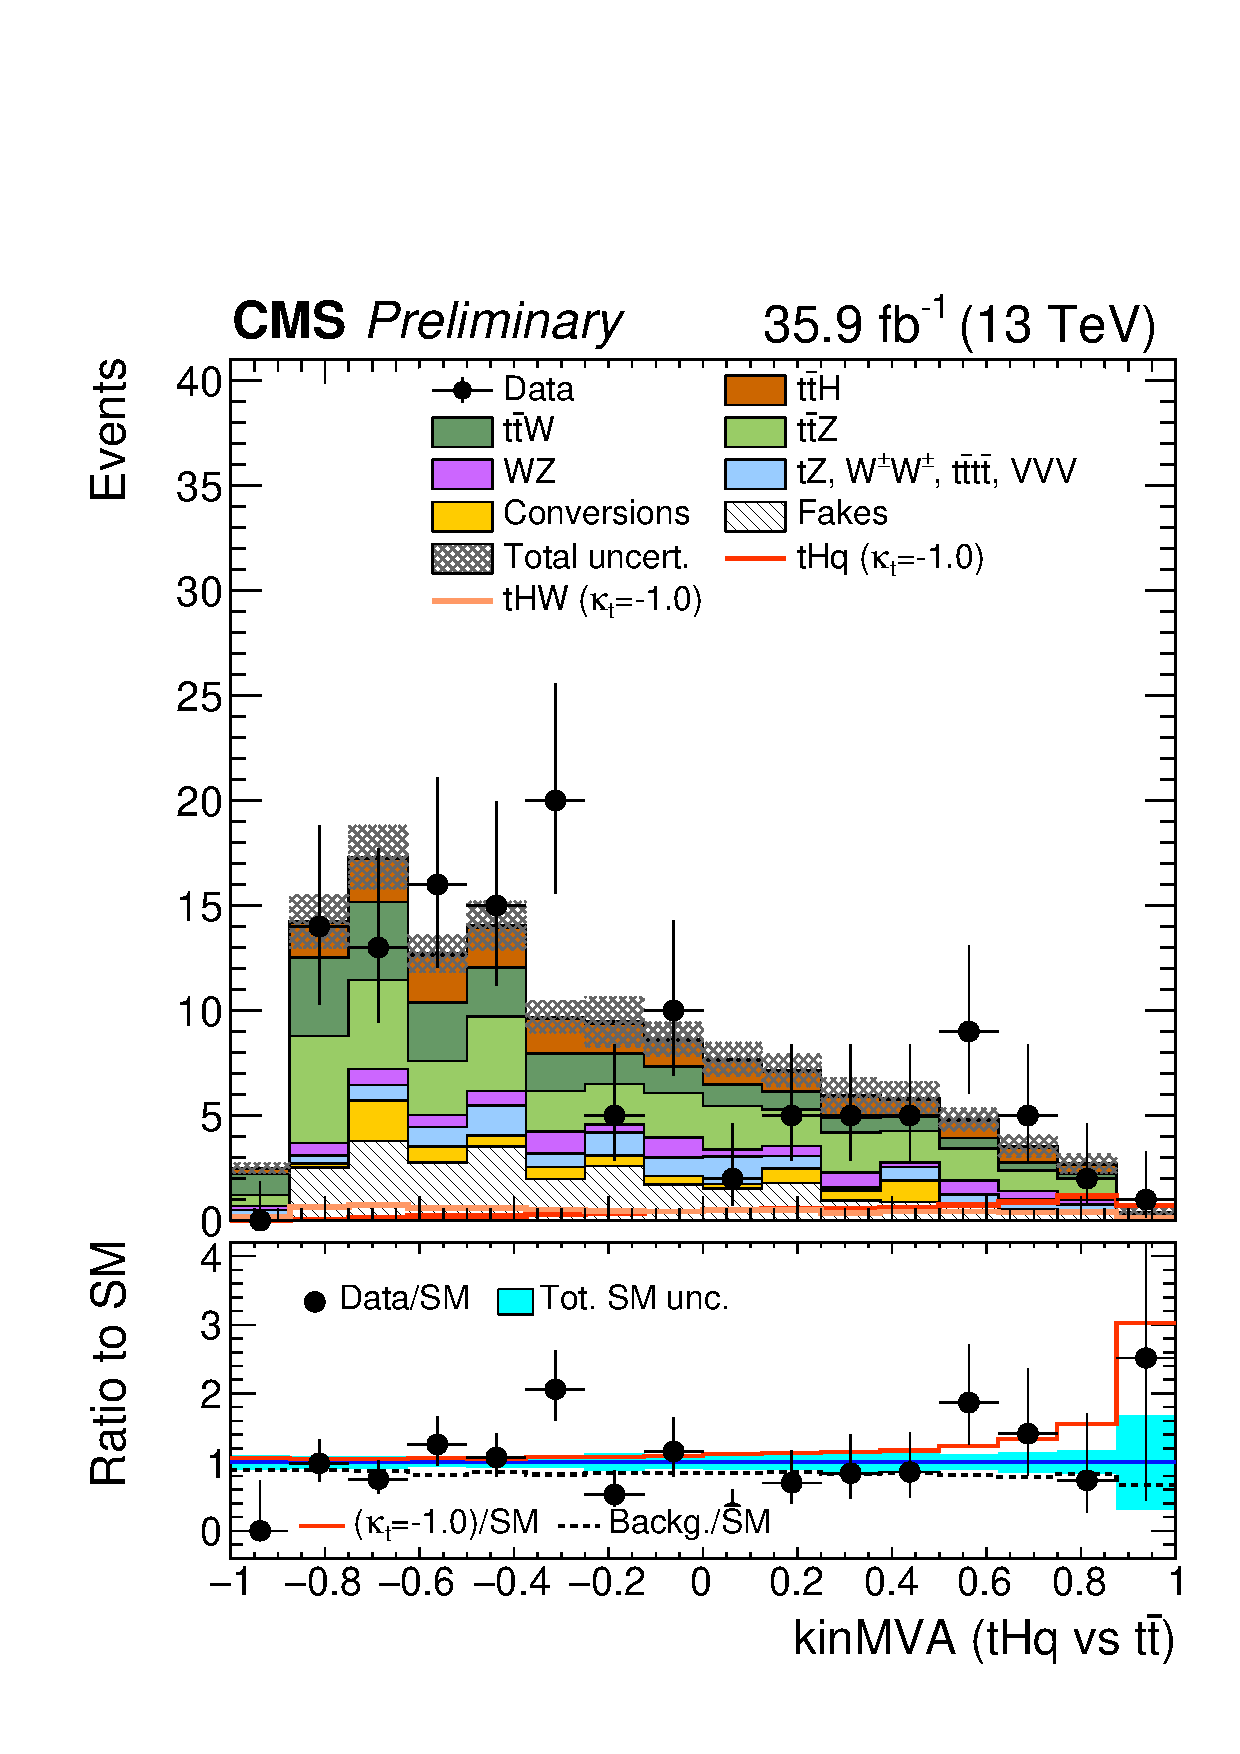
\includegraphics[width=0.32\textwidth]{Figures/polished/thqMVA_tt_3l_40_3l.pdf}
    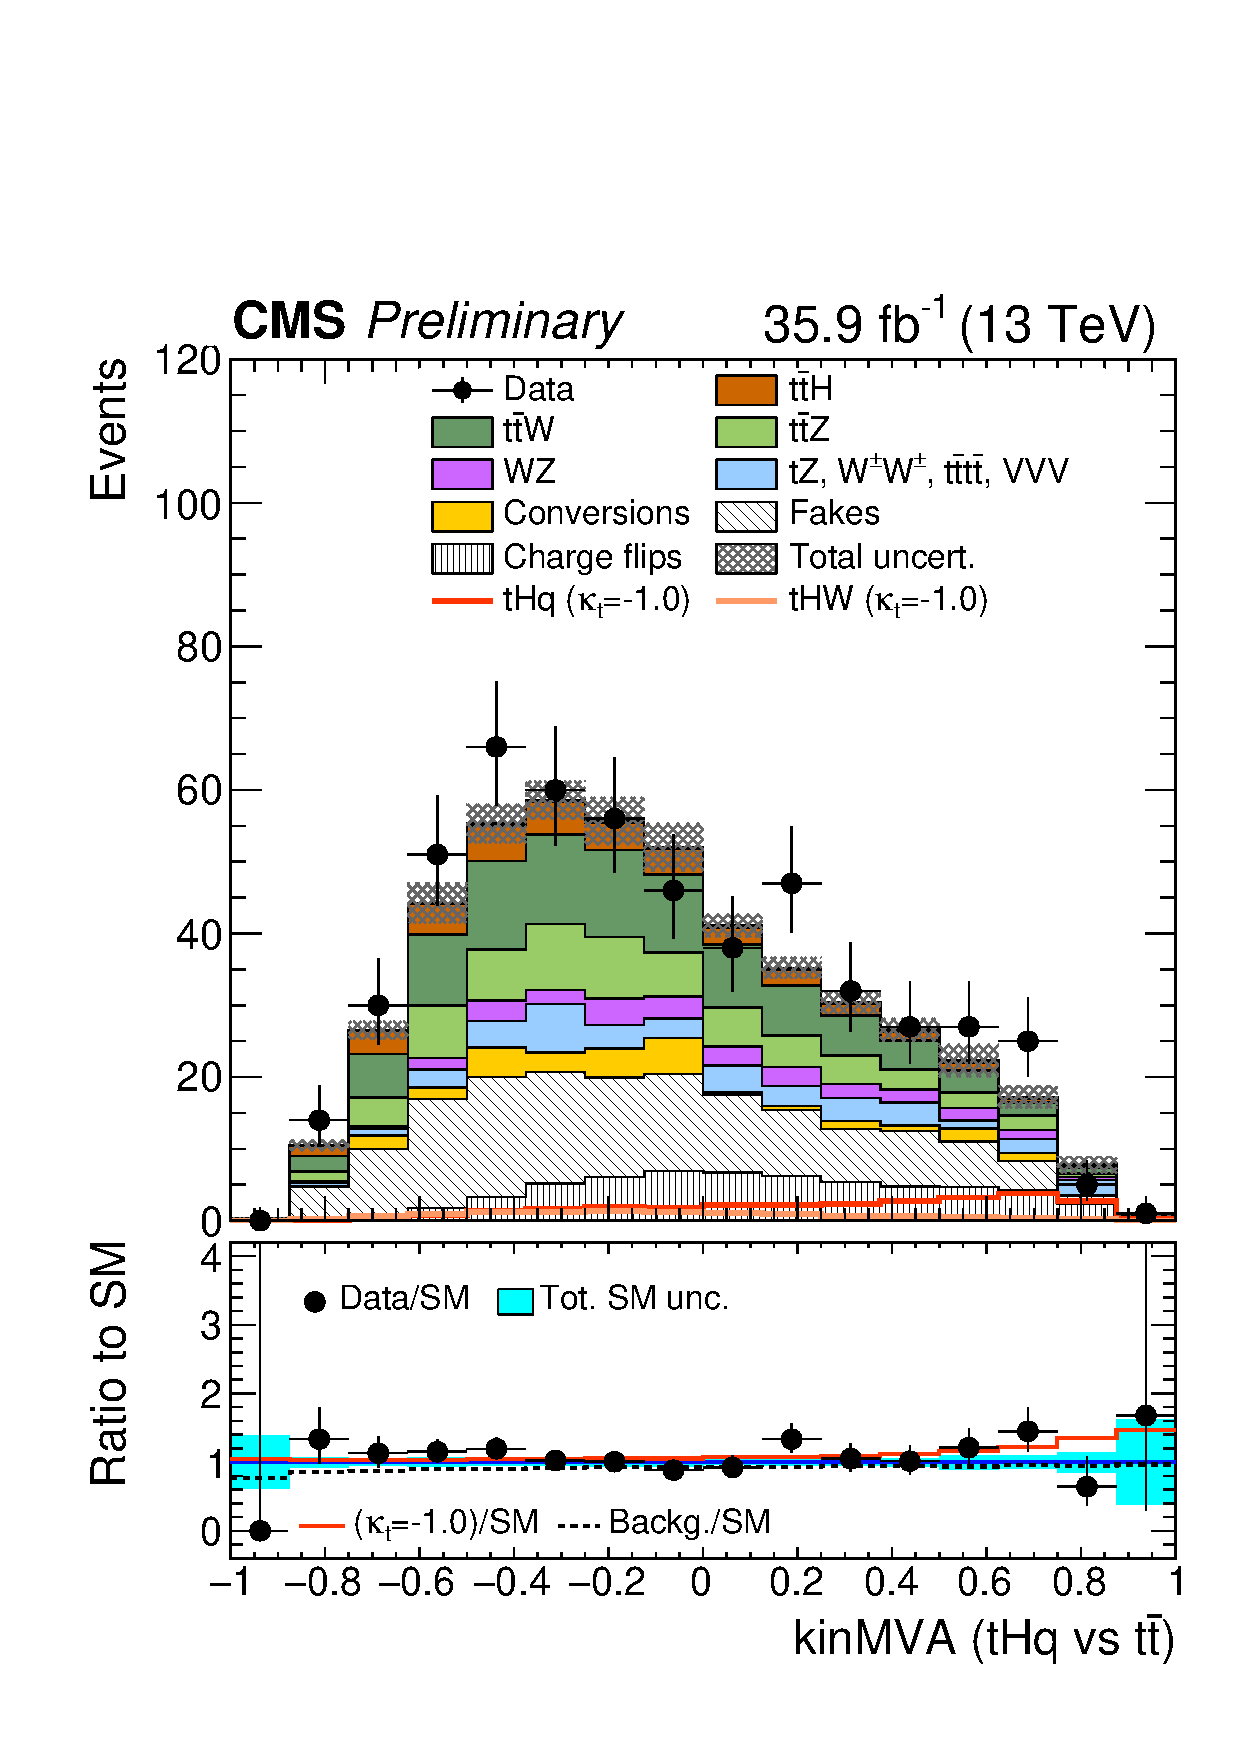
\includegraphics[width=0.32\textwidth]{Figures/polished/thqMVA_tt_2lss_40_em.pdf}
    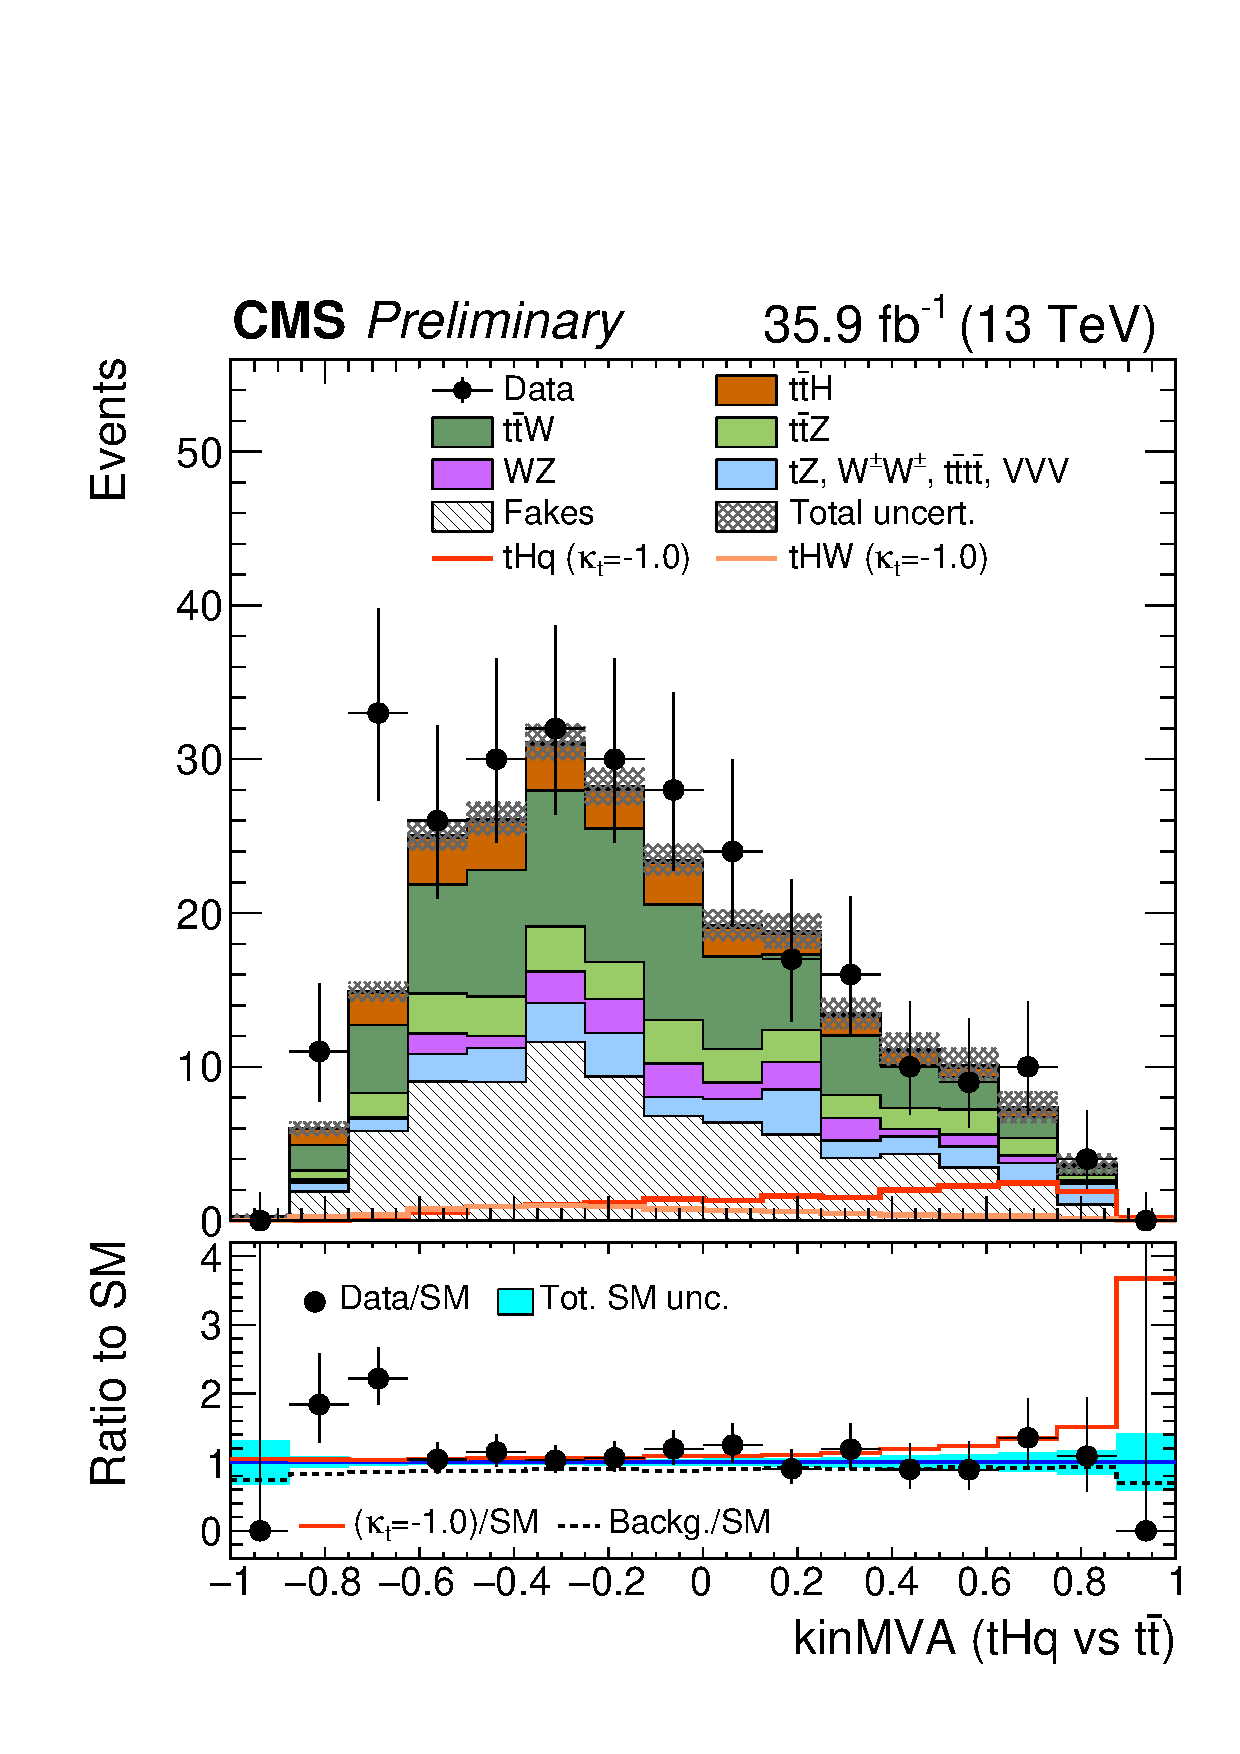
\includegraphics[width=0.32\textwidth]{Figures/polished/thqMVA_tt_2lss_40_mm.pdf}
  \end{center}
  \caption{Pre-fit BDT classifier outputs, for the three-lepton channel (left), \emu\ (center), and \mumu\ (right), for 35.9~\fbinv, for training against \ttV\ (top row) and against \ttbar\ (bottom row).
  In the box below each distribution, the ratio of the observed and predicted event yields is shown.
  The shape of the two \tH\ signals for $\Ct=-1.0$ is shown, normalized to their respective cross sections for $\Ct=-1.0, \CV=1.0$.
  The grey band represents the unconstrained (pre-fit) statistical and systematical uncertainties.\label{fig:postfitshapes}}
\end{figure}

\begin{figure}[!htb]
  \begin{center}
    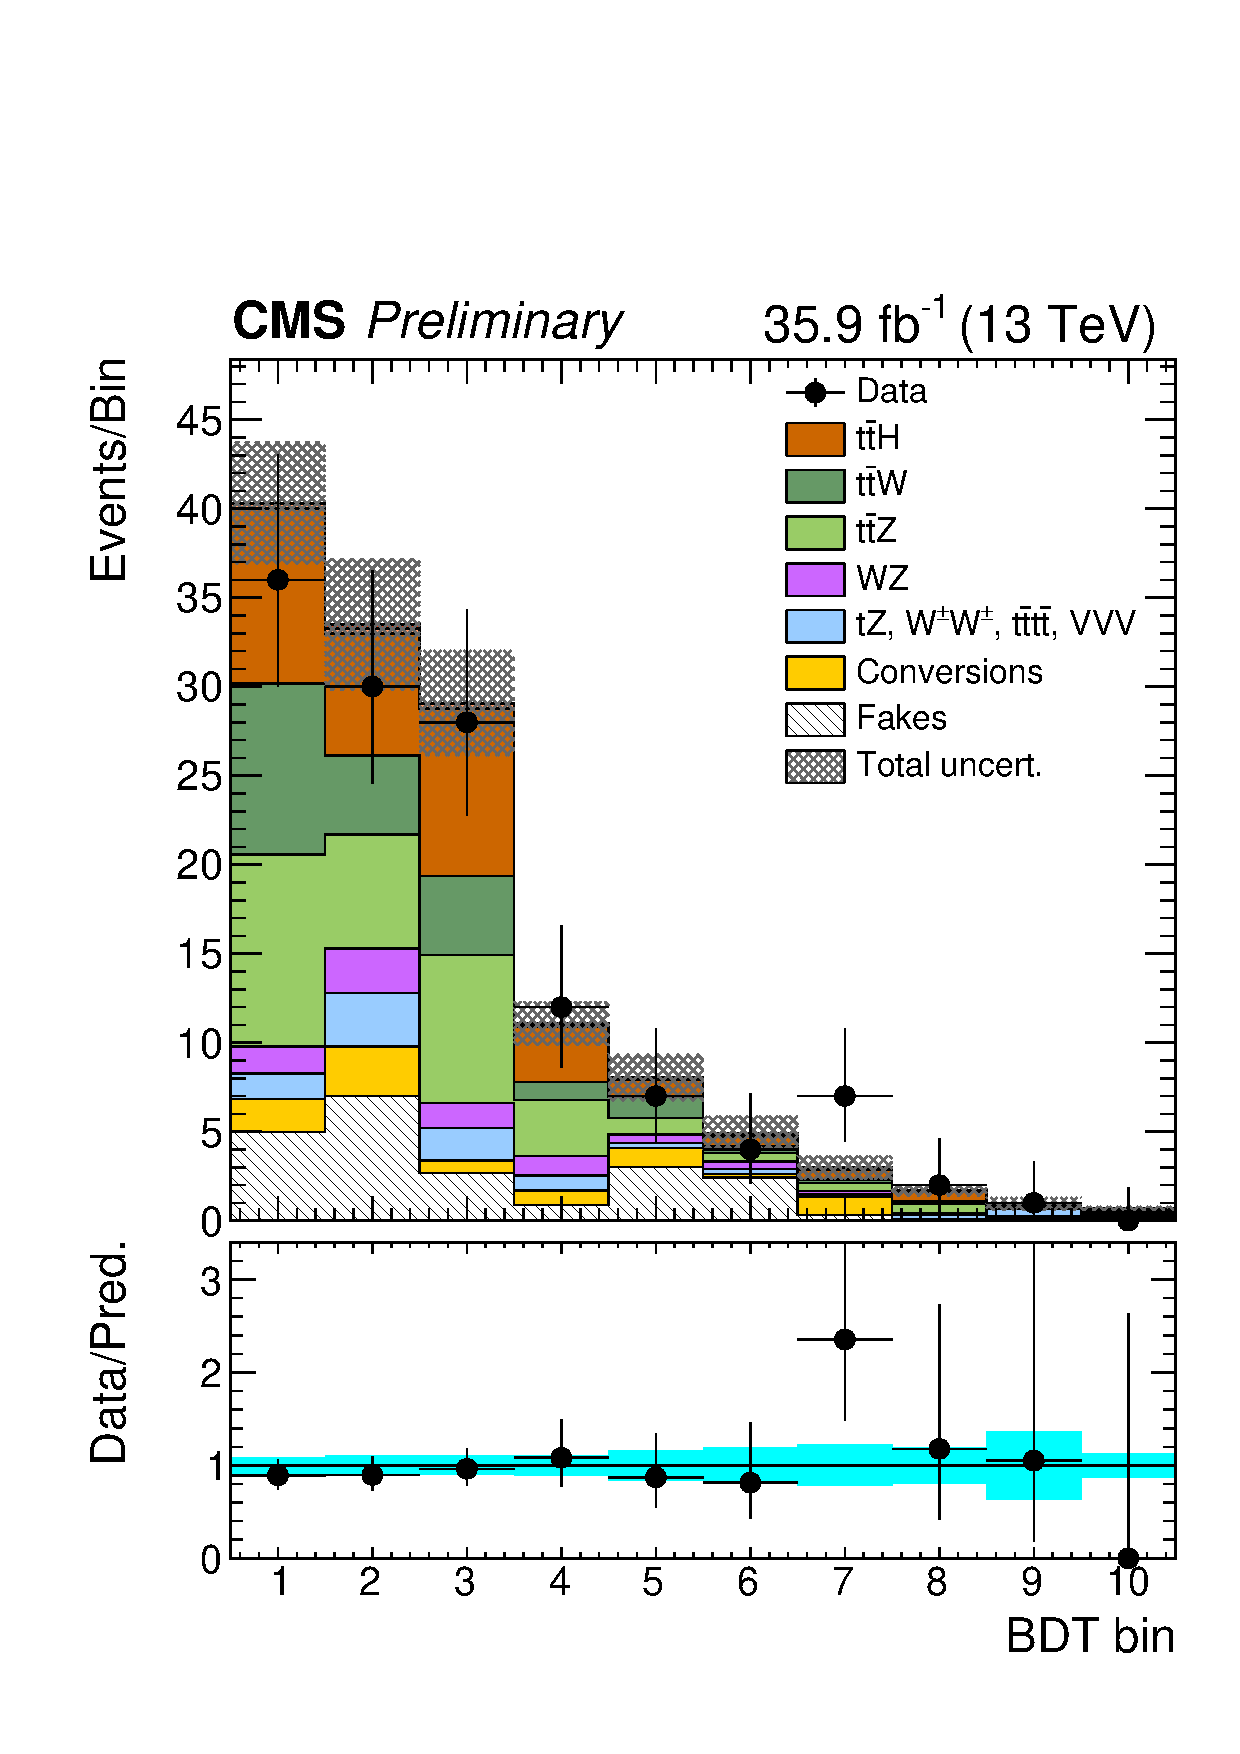
\includegraphics[width=0.32\textwidth]{Figures/postfit/tHq_3l_13TeV_fit_s.pdf}
    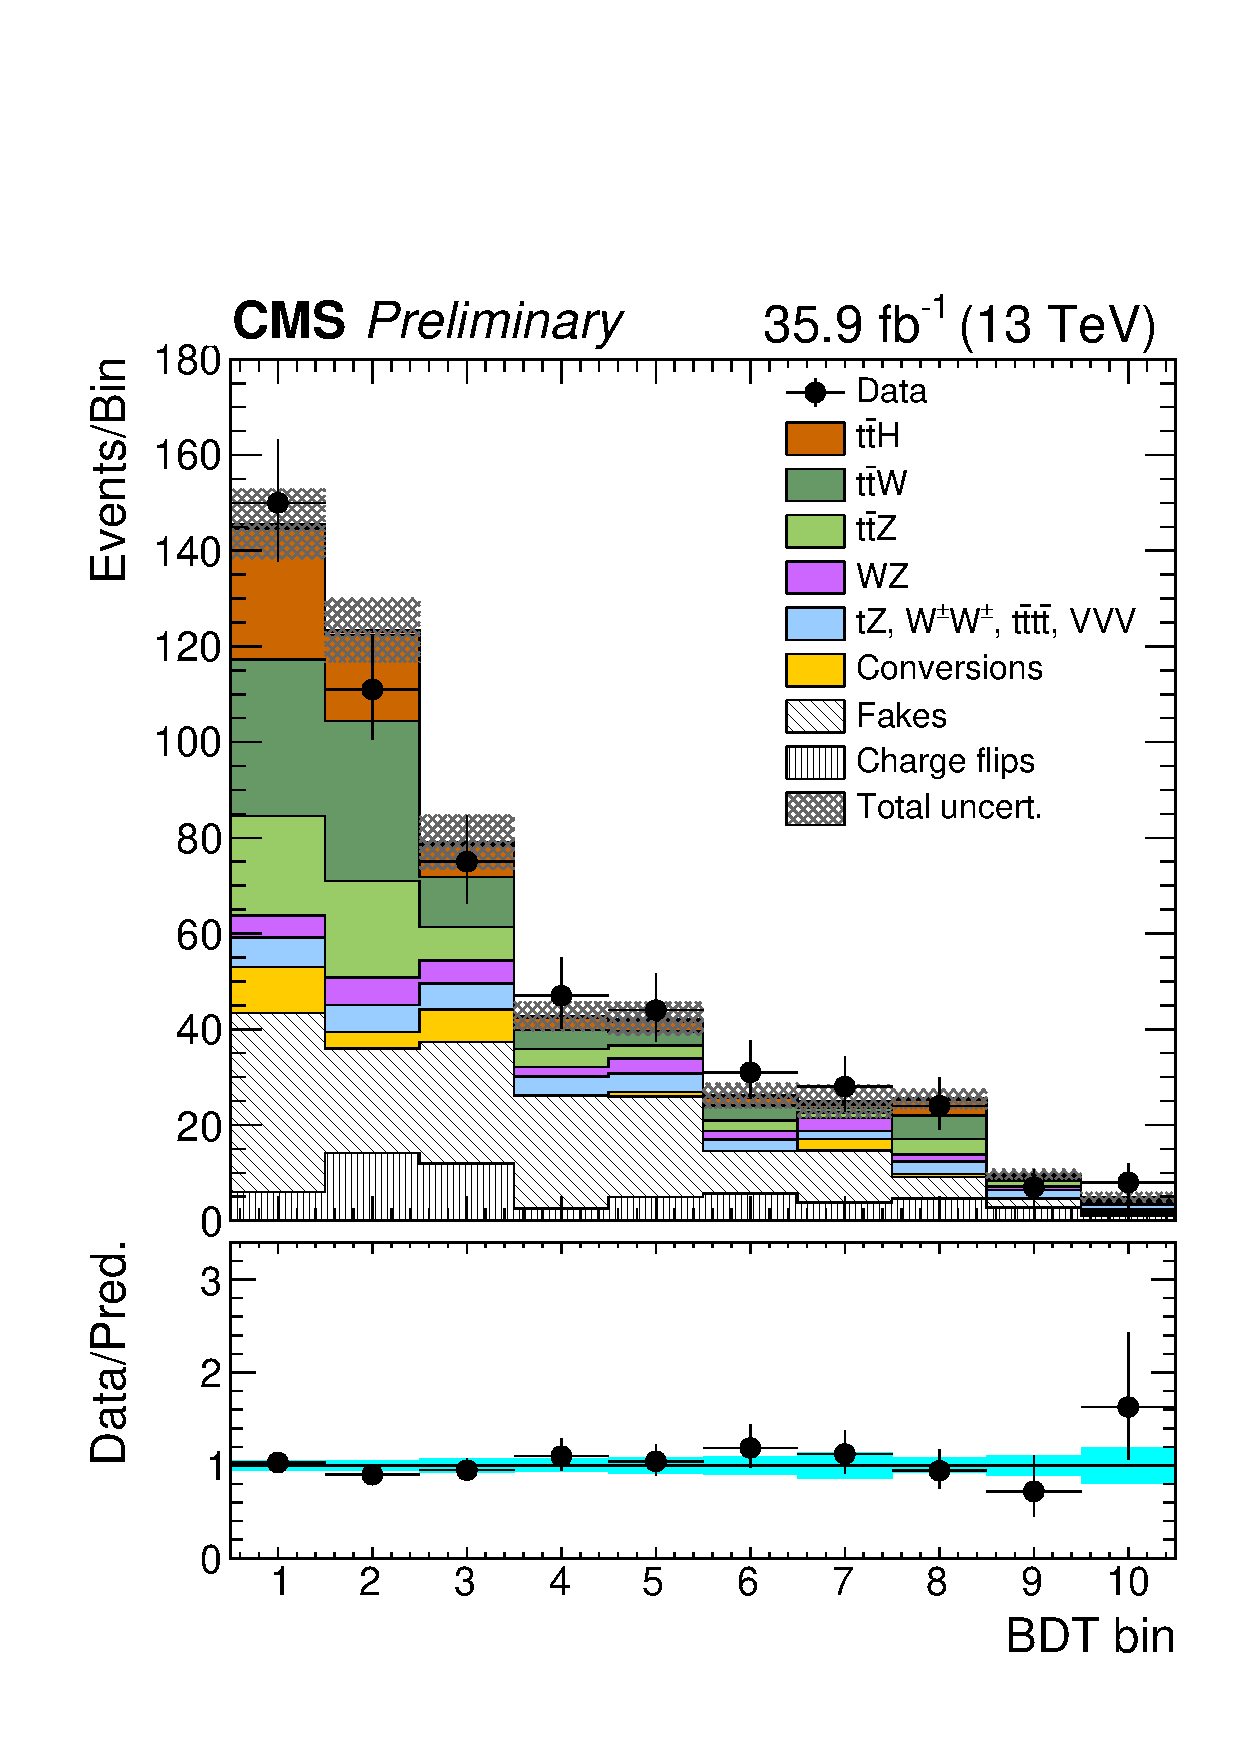
\includegraphics[width=0.32\textwidth]{Figures/postfit/tHq_2lss_em_13TeV_fit_s.pdf} 
    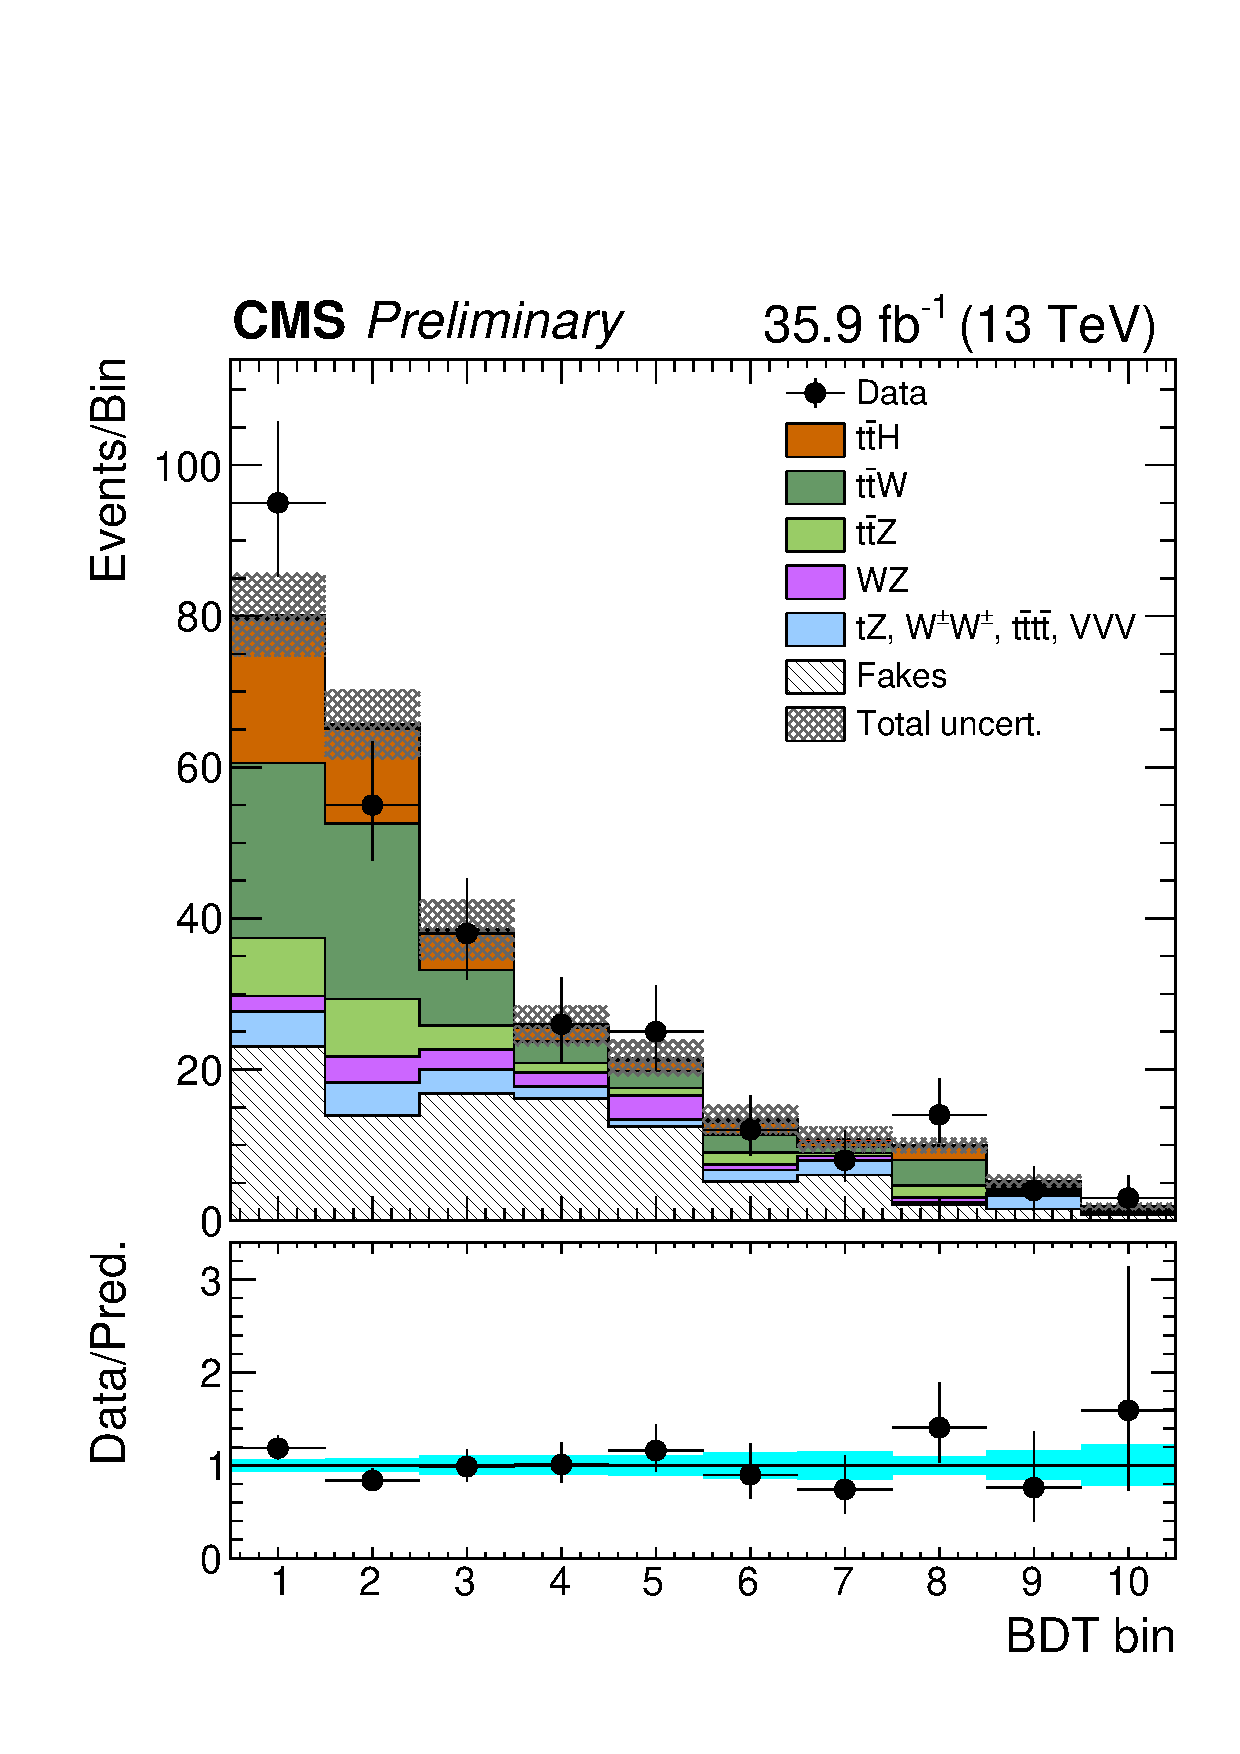
\includegraphics[width=0.32\textwidth]{Figures/postfit/tHq_2lss_mm_13TeV_fit_s.pdf}
  \end{center}
  \caption{Post-fit categorized BDT classifier outputs as used in the maximum likelihood fit for the three-lepton channel (left), \emu\ (center), and \mumu\ (right), for 35.9~\fbinv.
  In the box below each distribution, the ratio of the observed and predicted event yields is shown.
  % The grey band represents the unconstrained (pre-fit) statistical and systematical uncertainties.
  \label{fig:finalbins}}
\end{figure}

The observed 95\% C.L. upper limits on the $\tH+\ttH$ signal cross sections for the case of inverted couplings ($\Ct/\CV=-1.0$) for the individual channels are, respectively, $1.00$, $0.84$, and $0.70\,\mathrm{pb}$ for the \mumu, \emu, and trilepton final states, corresponding to $2.3$, $1.9$, and $1.6$ times the respective expected cross sections for $\CV=1.0$.
The combination of all three channels yields a limit of $0.64\,\mathrm{pb}$ on a signal shape expected for $\Ct/\CV=-1.0$, corresponding to $1.4$ times the expected $\tH+\ttH$ cross section with $\Ct=-1.0, \CV=1.0$.
% In this evaluation, all extra Higgs boson yields arising from the $\Ct=-1$ condition are considered as signal.
In the standard model scenario ($\Ct/\CV=1.0$), the observed upper limit on the cross section times branching ratio is $0.56\,\mathrm{pb}$, corresponding to $3.1$ times the expected SM cross section of $\tH+\ttH$.
Table~\ref{tab:limits} summarizes the results for the inverted coupling scenario and for the standard model.

The best-fit combined signal strength for the standard model hypothesis is $1.8\,\pm\,0.3\mathrm{(stat.)}\,\pm\,0.6\mathrm{(syst.)}$, corresponding to an observed significance of $2.7\sigma$ ($1.5\sigma$ expected) over a background-only hypothesis.
For a scenario of inverted couplings ($\Ct=-1=-\CV$), the best fit signal strength is $0.7\pm0.4$, corresponding to a significance of $1.7\sigma$ ($2.5\sigma$ expected), whereas the fit prefers a signal strength compatible with $0$ for a scenario with $\Ct=0$ (where the \ttH\ component vanishes).

The expected and observed limits are shown in Fig.~\ref{fig:limits} as a function of $\Ct/\CV$. %  and their 68\% and 95\% C.L. uncertainty ranges,
Comparing the observed upper limit with the theoretical prediction of the $\tH+\ttH$ cross section times BR for $\CV=1.0$ constrains the allowed range of coupling configurations $\Ct/\CV$ to between about $-1.25$ and $+1.60$.

\begin{table}[h!]
  \begin{center}
    \begin{tabular}{llcccc} \hline 
      Scenario  & Channel  & Obs. Limit    & \multicolumn{3}{c}{Exp. Limit (pb)}         \\
                &          & (pb)          & Median        & $\pm1\sigma$ & $\pm2\sigma$ \\ \hline \hline
   $\Ct/\CV=-1$ & \mumu\   & 1.00          &         0.58  & [0.42, 0.83] & [0.31, 1.15] \\
                & \emu\    & 0.84          &         0.54  & [0.39, 0.76] & [0.29, 1.03] \\
                & \threel\ & 0.70          &         0.38  & [0.26, 0.56] & [0.19, 0.79] \\ 
                & Combined & \textbf{0.64} & \textbf{0.32} & [0.22, 0.46] & [0.16, 0.64] \\ \hline
    $\Ct/\CV=1$ & \mumu\   & 0.87          &         0.41  & [0.29, 0.58] & [0.22, 0.82] \\
    (SM-like)   & \emu\    & 0.59          &         0.37  & [0.26, 0.53] & [0.20, 0.73] \\
                & \threel\ & 0.54          &         0.31  & [0.22, 0.43] & [0.16, 0.62] \\
                & Combined & \textbf{0.56} & \textbf{0.24} & [0.17, 0.35] & [0.13, 0.49] \\ \hline
    \end{tabular}
    \caption{Expected and observed 95\% C.L. upper limits on the $\tH+\ttH$ production cross section times $\PH\to\W\W^*+\tautau+\Z\Z^*$ branching ratio for a scenario of inverted couplings ($\Ct/\CV=-1.0$, top rows) and for a standard-model-like signal ($\Ct/\CV=1.0$, bottom rows), in pb. The expected limit is calculated on a background-only MC dataset. % and quoted with $\pm$1$\sigma$ and $\pm$2$\sigma$ probability ranges.
    \label{tab:limits}}
  \end{center}
\end{table}

\begin{figure}[!h]
  \centering
  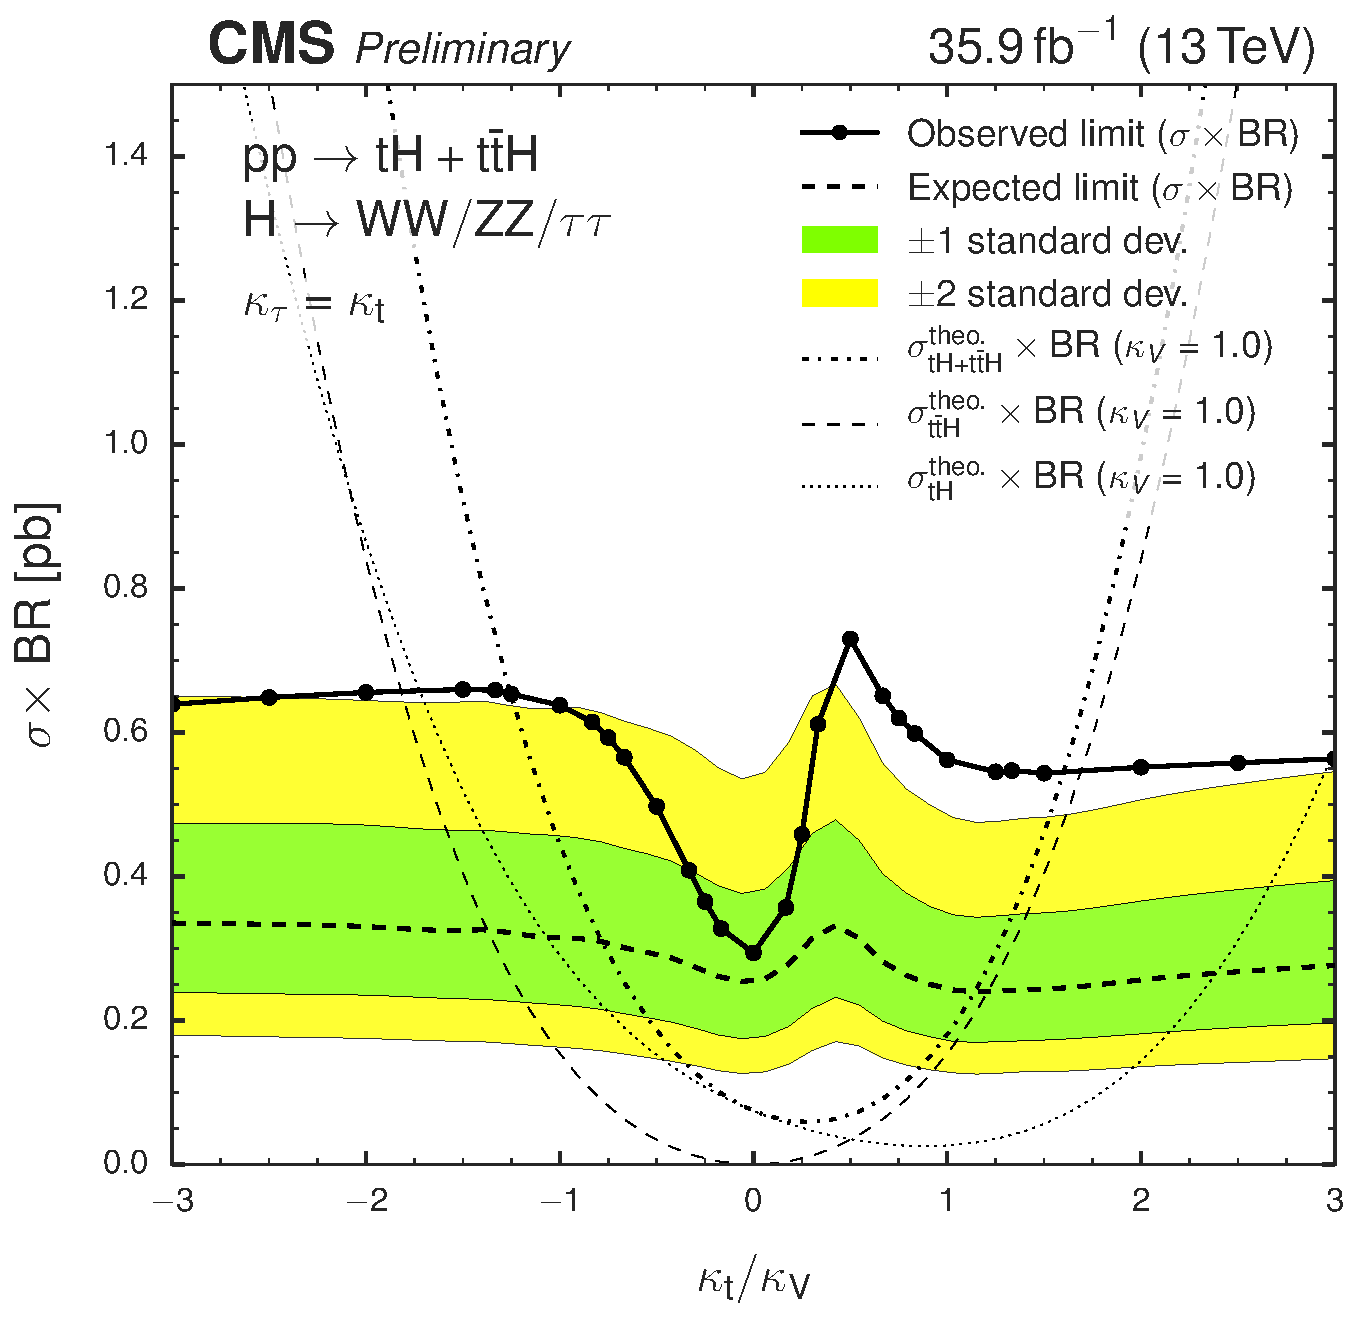
\includegraphics[width=0.8\textwidth]{Figures/xs_limits_K6.pdf}
  \caption{Observed and expected 95\% C.L. upper limit on the $\tH+\ttH$ cross section times $\PH\to\W\W^*+\tautau+\Z\Z^*$ branching fraction for different values of the coupling ratio \Ct/\CV. The expected limit is derived from a background-only MC dataset. % and shown with its $\pm1\sigma$~(green) and $\pm2\sigma$~(yellow) probability bands.
  \label{fig:limits}}
\end{figure}

The sensitivity of the analysis is limited by systematic uncertainties, predominantly by those concerning the normalizations of the main background components (the non-prompt lepton estimation, the scale uncertainties for $\ttW$ and $\ttZ$), as well as by the uncertainties on the measured lepton efficiency.
